\section{Group actions on CAT(0) cube complexes and strong group boundaries}
\label{sec:group}

\subsection{Extending the group action to the Roller boundary}
\label{sec:ga-roller}

In this section I would like to remark on how one can extend a group action on a CAT(0) cube complex \(X\) to its Roller boundary \(\bar X\). For that matter, let in the following \(\Gamma\) be a discrete countable group with an action \(\Gamma \to \Aut(X)\), where \(X\) is a finite dimensional CAT(0) cube complex. \(Aut(X)\) consists of the combinatorial isomorphisms (c.\,.f.\ Def.~\ref{def:morphism-ccc}).

The following proposition collects some facts about how cubical isomorphisms act on \(X\).

\begin{prop}
  Let \(g \in \Aut(X)\). Then there holds
  \begin{enumerate}
  \item \(\mathfrak{\hat h} \in \mathcal{\hat H}(X) \Rightarrow  g\mathfrak{\hat h} \in \mathcal{\hat H}(X)\)
  \item \(\mathfrak{h} \in \mathcal{H}(X) \Rightarrow  g\mathfrak{h} \in \mathcal{H}(X)\)
  \item \(\forall \mathfrak{h} \in \mathcal{H}(X)\colon g(\mathfrak{h}^\ast) = (g\mathfrak{h})^\ast\)
  \item \(\mathfrak{h,h'} \in \mathcal{H}(X)\colon \mathfrak{h} \subset \mathfrak{h'} \Rightarrow g\mathfrak{h} \subset g\mathfrak{h'}\)
  \item \(\alpha \in \bar X \Rightarrow g\alpha \in \bar X\)
  \item If \(\alpha\) satisfies the descending chain condition then so does \(g\alpha\).
  \end{enumerate}
\end{prop}

\begin{proof}
  1.\ is an immediate consequence of the fact, that \(g\) is an isometry. This leads directly to 2 and 3. For 4.\ we only need that \(g\) is a bijection and 5 and 6 are then simple applications of 4.
\end{proof}

With the above proposition in place we already see that each group action \(\Gamma \to \Aut(X)\) immediately leads to an action \(\Gamma \to \operatorname{Perm}(\bar X)\). However, this is not yet what we want. It would be preferable, if the image lay in the homeomorphisms of \(X\). This will be accomplished with the next lemma.

\begin{lemma}
  Let \(g \in \Aut(X)\) and \(\mathcal{U} \coloneqq \mathcal{U}(\mathfrak{h}_1, \dots, \mathfrak{h}_n) \subset \bar X\) a basic open set. Then we have
  \[
    g^{-1} \mathcal{U} = \mathcal{U}(g^{-1}\mathfrak{h}_1, \dots, g^{-1}\mathfrak{h}_n).
  \]
  Hence, \(g \in \operatorname{Homeo}(\bar X)\).
\end{lemma}

Together we arrive at the following result.

\begin{thm}
  \label{thm:roller-action}
  Let \(\Gamma\) be a group and \(\Gamma \to \Aut(X)\) a group action on a CAT(0) cube complex \(X\). Then this action extends to an action \(\Gamma \to \operatorname{Homeo}(\bar X)\) on the Roller compactification.
\end{thm}

\subsection{Special group actions on CAT(0) cube complexes}
\label{sec:special}

\begin{defin}[(Non-)elementary action]
  A group action \(\Gamma \to \Aut(X)\) is called \emph{elementary}, if there exists a finite orbit of the action on \(X \sqcup \partial_{\sphericalangle}X\). Otherwise the action is called \emph{non-elementary}.
\end{defin}


The above definition has one interesting immediate consequence:
\begin{prop}
  \label{prop:ne-unbounded}
  If \(\Gamma \to \Aut(X)\) acts non-elementary on \(X\), then \(X\) is unbounded.
\end{prop}

\begin{bsp}
  The previous observation already provides many example for elementary actions by considering any group action on a finite cube complex.

  Another example is \(X \coloneqq \R^d\) with its standard cubulation and any cyclic subgroup of \(\Z^d\) acting by translations. This action has no finite orbits in \(\R^d\), but every point at infinity is fixed. Indeed, two rays define the same point at infinity if and only if they are parallel. However, a translated ray is still parallel to the untranslated ray.

  As an example for a non-elmentary action, we consider an infinite complete binary tree \(X\). That means we have a root vertex \(r\) which has exactly two children and each child has gain exactly two children and so forth. We consider the group \(\Gamma\) acting on \(X\) generated by the following operations: Reflection and rotation at arbitrary vertices. Reflection switches the two subtrees of a vertex and rotation replaces itself with one of its children and the parent moving further down in the tree. The idea of these generating operations can be found in Figures~\ref{fig:rotation} and~\ref{fig:reflection}.

  \begin{figure}[htbp]{}
    \centering
    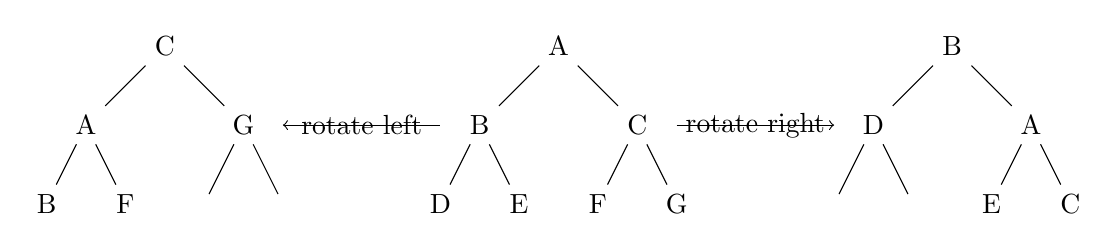
\begin{tikzpicture}
    \node (C'') at ( 0, 0) {C};
    \node (A'') at (-1,-1) {A};
    \node (G'') at ( 1,-1) {G};
    \node (B'') at (-1.5,-2) {B};
    \node (F'') at (-0.5,-2) {F};
    \node (E'') at ( 0.5,-2) {};
    \node (D'') at ( 1.5,-2) {};
    \draw (C'') -- (A'')
    (C'') -- (G'')
    (A'') -- (B'')
    (A'') -- (F'')
    (G'') -- (D'')
    (G'') -- (E'');

    \draw [<-] (1.5,-1) -- node {rotate left} (3.5,-1);
  \begin{scope}[shift={(5,0)}]
  \node (A) at ( 0, 0) {A};
  \node (B) at (-1,-1) {B};
  \node (C) at ( 1,-1) {C};
  \node (D) at (-1.5,-2) {D};
  \node (E) at (-0.5,-2) {E};
  \node (F) at ( 0.5,-2) {F};
  \node (G) at ( 1.5,-2) {G};
  \draw (A) -- (B);
  \draw (A) -- (C);
  \draw (B) -- (D)
  (B) -- (E)
  (C) -- (F)
  (C) -- (G);
  \draw [->] (1.5,-1) -- node {rotate right} (3.5,-1);
  \begin{scope}[shift={(5,0)}]
    \node (B') at ( 0, 0) {B};
    \node (D') at (-1,-1) {D};
    \node (A') at ( 1,-1) {A};
    \node (F') at (-1.5,-2) {};
    \node (G') at (-0.5,-2) {};
    \node (E') at ( 0.5,-2) {E};
    \node (C') at ( 1.5,-2) {C};
    \draw (B') -- (D')
    (B') -- (A')
    (A') -- (E')
    (A') -- (C')
    (D') -- (F')
    (D') -- (G');
  \end{scope}
    
  \end{scope}

\end{tikzpicture}

%%% Local Variables:
%%% mode: latex
%%% TeX-master: "../Master"
%%% End:

    \caption{Rotation of a binary (sub-)tree}
    \label{fig:rotation}
  \end{figure}

  \begin{figure}[htbp]
    \centering
    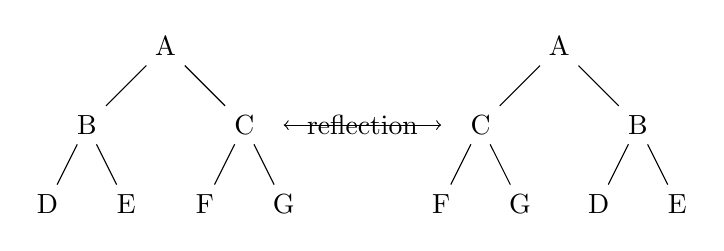
\begin{tikzpicture}
  \node (A) at (0,0) {A};
  \node (B) at (-1,-1) {B};
  \node (C) at ( 1,-1) {C};
  \node (D) at (-1.5,-2) {D};
  \node (E) at (-0.5,-2) {E};
  \node (F) at ( 0.5,-2) {F};
  \node (G) at ( 1.5,-2) {G};
  \draw
  (A) -- (B)
  (A) -- (C)
  (B) -- (D)
  (B) -- (E)
  (C) -- (F)
  (C) -- (G);
  \draw[<->] (1.5,-1) -- node {reflection} (3.5,-1);
  \begin{scope}[shift={(5,0)}]
  \node (A') at (0,0) {A};
  \node (B') at ( 1,-1) {B};
  \node (C') at (-1,-1) {C};
  \node (D') at ( 0.5,-2) {D};
  \node (E') at ( 1.5,-2) {E};
  \node (F') at (-1.5,-2) {F};
  \node (G') at (-0.5,-2) {G};
  \draw
  (A') -- (B')
  (A') -- (C')
  (B') -- (D')
  (B') -- (E')
  (C') -- (F')
  (C') -- (G');
  \end{scope}
\end{tikzpicture}

%%% Local Variables:
%%% mode: latex
%%% TeX-master: "../Master"
%%% End:

    \caption{Reflection of a binary (sub-)tree}
    \label{fig:reflection}
  \end{figure}
  We first check, that we have no finite orbit in \(X\) itself. This can be established via the rotation. Taking any vertx \(v\) we can rotate around this vertex multiple times and with each one the original \(v\) will be pushed deeper down the tree. Hence, every orbit contains infinitely many points. In order to see that there are no finite orbits at infinity, we need to check when to geodesic rays have bounded distance from one another. However, in a tree this is only the case if they coincide after finitely many steps. Hence, every geodesic ray has a unique representative emanating from the root \(r\). Choosing any such geodesic ray, we can generate infinitely many inequivalent ones by reflecting at vertices traversed by it, showing again that there is no finite orbit.
\end{bsp}


\begin{defin}[Essential action]
  A group action \(\Gamma \to \Aut(X)\) is called \emph{essential}, if the essential core of \(\Gamma\) is the whole space \(X\).
\end{defin}

\begin{bsp}
  Consider \(X\coloneqq \R^d\) with the standard cubulation and the action of \(\Gamma \coloneqq \Z^d\) on it via translations. This action respects the cube complex structure. Additionally, every hyperplane in \(X\) is a hyperplane \(\mathfrak{\hat h} \in \mathcal{\hat H}(X)\) in the usual Euclidean sense and of course choosing any vertex \(v\) its translates get arbitrarily far away from \(\mathfrak{h}\) on either side. Hence \(\Gamma\) acts essentially on \(X\).
\end{bsp}

\subsection{Strong \(\Gamma\)-boundaries}
\label{sec:grp-boundary}

\begin{defin}
  A measurable space \((B, \Sigma)\) is called a \emph{standard Borel space}, if it is isomorphic (as a measurable space) to a measurable set \(E \subset X\), where \(X\) is a complete separable metric space equipped with its Borel \(\sigma\)-algebra.

  A measure space \((B, \Sigma, \mu)\) is called a \emph{Lebesgue space}, if it is a standard Borel space and \(\mu\) is a regular probability measure.

  Let \((B, \Sigma)\) be a measurable space. We can define an equivalence relation on all measures on \(\Sigma\) via \(\mu \sim \nu\) if and only if the null-sets of \(\mu\) and \(\nu\) coincide. An equivalence class \([\mu]\) is called a \emph{measure class}. If a group \(\Gamma\) acts measurably on \(B\), then \(\Gamma\) is said to \emph{preserve measure classes}, if for every measure \(\mu\) of \(\Sigma\) we have that \(\mu(B) = 0\) implies that \(\mu(g^{-1} B) = 0\) for every \(B \in \Sigma\) and \(g \in \Gamma\).
\end{defin}

\begin{defin}[Amenable group action]
  Let \(E\) be a separable Banach space. Then I denote by \(E^\ast_1\) the unit ball in its dual space. Let \(S\) be a standard Borel space and for each \(s \in S\) consider \(A_s \subset E^\ast_1\) a non-empty convex weak\(\ast\)-compact subspace. Then \((A_s)_{s \in S}\) will be called a \emph{Borel field of compact convex sets} if \(\{(s, \lambda) \mid \lambda \in A_s\}\) is a Borel subset of \(S \times E^\ast_1\).

  Let \(\Gamma\) be a locally compact group with a measure class preserving group action on \(S\). Furthermore, let \(M\) be a Borel group. Then \(\alpha \colon \Gamma \times s \to M\) is called a \emph{(left) cocycle} if \(\alpha(gh, s) = \alpha(g, hs) \alpha(h, s)\) for all \(g, h \in \Gamma\) and almost all \(s \in S\).

  Each element \(T\) of \(\Isom(E)\) gives rise to a homeomorphism \(T^\ast\) of \(E^\ast_1\) via \((T^\ast\Phi)(x) \coloneqq \Phi(Tx)\) for every \(x \in E\). Thus every cocycle \(\alpha \colon S \times \Gamma \to \Isom(E)\) gives rise to a cocycle \(\alpha^\ast \colon S \times \Gamma \to \operatorname{Homeo}(E^\ast)\) via \(\alpha^\ast (g, s) = (\alpha(g, s)^{-1})^\ast\). A Borel field \((A_s)_{s \in S}\) is called \emph{\(\alpha\)-invariant} if \(\alpha^\ast(g, s) A_{s} = A_{gs}\) for each \(g \in \Gamma\) and almost all \(s \in S\).
  
  Let \(\Gamma\) be a locally compact group and \(S\) a standard Borel space with measure class preserving Borelian \(\Gamma\)-action. The \(\Gamma\)-action is said to be \emph{amenable} if for every separable Banach space \(E\), every Borelian (left) cocycle \(\alpha \colon S \times G \to \Isom(E)\) and every \(\alpha\)-invariant Borel field \((A_s)_{s \in S}\), there exists a Borel map \(\phi \colon S \to E^\ast_1\) such that \(\phi(s) \in A_s\) for almost all \(s\) and for each \(g \in \Gamma\) we have \(\alpha^\ast(g, s) \phi(s) = \phi(gs)\) almost everywhere.
\end{defin}

\begin{defin}[(Doubly) ergodic action]
  Let \((B, \Sigma, \mu)\) be a probability space with a measurable group action by \(\Gamma\). Then the action is called \emph{ergodic} if one of the two equivalent conditions is satisfied:
  \begin{enumerate}
  \item For every \(E \in \Sigma\) such that \(g^{-1}E = E\) for each \(g \in \Gamma\) we have \(\mu(E) = 0\) or \(\mu(E) = 1\) or
  \item every measurable \(\Gamma\)-equivariant map \(f\colon B \to \R\) is essentially constant.
  \end{enumerate}
  The action is called \emph{doubly ergodic} if the diagonal action on \(B \times B\) equipped with the product measure is ergodic.
\end{defin}

\begin{bsp}
  Consider the Bernoulli space \(B \coloneqq \{0,1\}^{\Z}\) with the product \(\sigma\)-algebra stemming from the discrete topology on each of the sets \(\{0,1\}\). We equip this space with the measure \(\mu\), comming from the uniform distribution on each factor. Lastly, we let \(\Z\) act on this space via a shift operation. Then \textcite[Example 20.26]{Klenke} shows that this system is ergodic.
\end{bsp}

\begin{prop}
  \label{prop:coeff-ergodic}
  Every doubly ergodic action is automatically ergodic.
\end{prop}

\begin{proof}[Sketch]
  Consider the second criterion together with the (equivariant, measurable and non-constant) projection from the product to the first factor.
\end{proof}

\begin{lemma}
  \label{lemma:ergodicity-pushforward}
  Let \(A\) and \(B\) be measurable spaces with a measurable group action \(\Gamma\). Furthermore, let \(f\colon A \to B\) be a measurable \(\Gamma\)-equivariant map and \(\mu\) a measure on \(A\). If \(\Gamma\) acts ergodically on \((A, \mu)\) then \(\Gamma\) acts ergodically on \((B, f_\ast \mu)\).
\end{lemma}

\begin{proof}
  We will apply the first criterion for ergodicity. Let \(E \subset B\) be measurable such that \(g^{-1} E = E\) for every \(g \in \Gamma\). Then we have
  \[
    f^{-1}(E) = f^{-1}(g^{-1}E) = g^{-1}f^{-1}(E)
  \]
  because of the equivariance. Thus by the ergodicity on \(A\) we have \(\mu(f^{-1}(E))= 0\) or \(\mu(f^{-1}(E)) = 1\). However, \(\mu(f^{-1}(E))\) is exactly the definition of \(f_\ast\mu(E)\).
\end{proof}

\begin{defin}[Doubly ergodic action with coefficients]
  Let \(\Gamma\) be a group and \((B, \Sigma, \vartheta)\) a Lebesgue space endowed with a measure class preserving \(\Gamma\)-action. The action of \(\Gamma\) on \(B\) is \emph{doubly ergodic with coefficients} if any weak\(\ast\)-measurable \(\Gamma\)-equivariant map \(B \times B \to E\) into the dual \(E\) of a separable Banach space on which \(\Gamma\) acts by isometries is essentially constant.
\end{defin}

\begin{prop}
  If a group action is doubly ergodic with coefficients it is doubly ergodic in the usual sense.
\end{prop}

\begin{proof}
  We choose \(E = \R\) and apply the second ergodicity criterion.
\end{proof}

\begin{lemma}[{\cite[Section~2.a]{Bader2006}}]
  \label{lem:coeff-product}
  If \(\Gamma\) acts doubly ergodic with coefficients on \(B\). Then for every measure preserving ergodic \(\Gamma\)-space \((X, \mu)\), the space \(B \times B \times X\) is ergodic.
\end{lemma}

\begin{defin}[Strong \(\Gamma\)-boundary]
  Let \(\Gamma\) be a locally compact group. A Lebesgue space \((B, \Sigma, \vartheta)\) is called a \emph{strong \(\Gamma\)-boundary}, if there is a measurable group action of \(\Gamma\) on \(B\) and this action is
  \begin{enumerate}
  \item amenable and
  \item doubly ergodic with coefficients.
  \end{enumerate}
\end{defin}

\begin{lemma}[{\cite[Thm.\ V.6.6]{Conway}}]
  If \(X\) is a compact metric space. Then \(C(X)\) is separable.
\end{lemma}

\begin{thm}
  Let \(B\) be a strong \(\Gamma\)-boundary and \(X\) a compact metric space with a continuous \(\Gamma\) action. Then there exists a \(\Gamma\)-equivariant measurable map \(\phi \colon B \to \mathcal{P}(X)\), where \(\mathcal{P}(X)\) is the set of all probability measures on \(X\).
\end{thm}

\begin{proof}
  Consider \(C(X)\) the space of continuous functions from \(X\) to \(\R\). Together with the supremum norm this is a Banach space, which (by the previous lemma) is also separable. Furthermore, there exists a group action of \(\Gamma\) on \(C(X)\) via \((gf)(x) = f(g^{-1}x)\) for each \(g \in \Gamma\), \(f \in C(X)\) and \(x \in X\). This action is clearly via isometries. Also for \(\mu \in \mathcal{P}(X)\) we define the action to be \((g\mu)(A) = \mu(g^{-1} A)\) for every \(g \in \Gamma\) and \(A \in \Sigma\). Then the dual pairing established in the Riesz-Markow representation theorem yields \(\langle gf, \mu\ \rangle = \langle f, g^{-1} \mu \rangle\) or in other words \(g^\ast = g^{-1}\).
  Next, consider
  \[
    \alpha: \Gamma \times B \to \Isom(C(X)), (g, b) \mapsto g.
  \]
  This is a left cocycle.
  Since \(X\) is compact, we have \(C(X) = C_0(X)\) and thus, using the Riesz-Markow representation theorem, we yield \(C(X)^\ast \cong M_{s}(X)\). By Corollary~\ref{cor:banach-alaoglu} we know that \(\mathcal{P}(X)\) is weak\(\ast\)-compact and contained in the unit ball of \(M_s(X)\). Furthermore, \(\mathcal{P}(X)\) is convex and non-empty (take any normalized Dirac measure), thus we can choose \(A_b = \mathcal{P}(X)\) for all \(b \in B\). This is in fact an \(\alpha\)-invariant Borel field. Since \(B\) is a strong \(\Gamma\)-boundary, the \(\Gamma\) action is amenable and we yield a measurable map \(\phi \colon B \to C(X)^\ast_1\) such that \(\phi(b) \in A_b = \mathcal{P}(X)\), i.\,e.\ \(\phi \colon B \to \mathcal{P}(X)\) (which is still measurable). Lastly, we have
  \begin{align*}
    \phi(gb) & = \alpha^\ast(g, b) \phi(b)\\
               & = \left(\alpha(g,b)^{-1}\right)^\ast \phi(b)\\
               & = \left ( g^{-1}\right)^\ast \phi(b)\\
               & = g\phi(b).
  \end{align*}
\end{proof}

\begin{cor}
  \label{cor:p(x)}
  Let \(X\) be a finite dimensional CAT(0) cube complex and \(\bar X\) its Roller compactification. Let \(\Gamma \to \Aut(X)\) be a discrete countable group acting on \(X\). Furthermore, let \(B\) be a strong \(\Gamma\)-boundary. Then there exists \(\Gamma\)-equivariant measurable map \(\phi\colon B \to \mathcal{P}(\bar X)\), where \(\mathcal{P}(\bar X)\) is the set of probability measures on \(\bar X\).
\end{cor}

\begin{proof}
  By Corollary~\ref{cor:comp-met} it was established that \(\bar X\) is a compact metrizable space. Furthermore, the \(\Gamma\)-action on \(X\) extends to a \(\Gamma\)-action on \(\bar X\)(c.\,f.\ Theorem~\ref{thm:roller-action}). Thus all conditions for the previous theorem are satisfied and we get the desired map \(\phi\colon B \to \mathcal{P}(\bar X)\).
\end{proof}

%%% Local Variables:
%%% mode: latex
%%% TeX-master: "../Master"
%%% End:
